\documentclass{beamer}
\usetheme{Warsaw}
\usepackage{beamerthemesplit}
\title{Why \LaTeX \ ??}
\author{SPACE}
\date{\today}

\begin{document}
\maketitle
%\frame{\titlepage}

\begin{frame}
\frametitle{\LaTeX}
\begin{itemize}
\item \LaTeX\ is a document preparation system for high-quality typesetting.
\item  It is most often used for medium-to-large technical or scientific documents but it can be used for almost any form of publishing.
\item Free and Universal.
\end{itemize}
\end{frame}

\begin{frame}
\frametitle{\LaTeX}
%\textbf{Donald Ervin Knuth} is a computer scientist and Professor at Stanford University
%\framebox{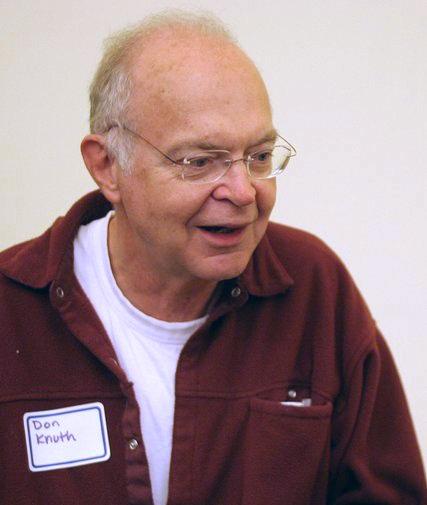
\includegraphics[width=1.5in]{knuth}}
\begin{columns}[c]
\column{1.5in}
\begin{itemize}
\item \textbf{Donald Ervin Knuth} is a computer scientist and Professor at Stanford University
\item Knuth is the creator of the TeX computer typesetting system
\end{itemize}
\column{1.5in}
\framebox{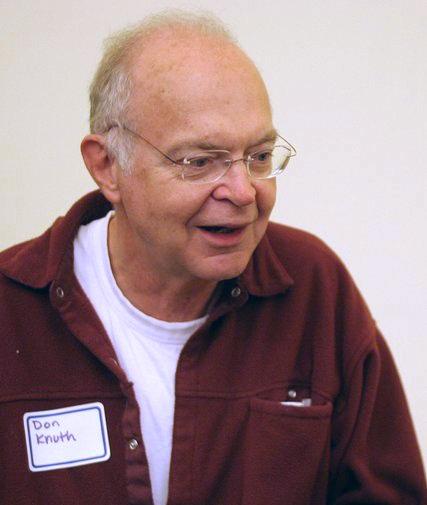
\includegraphics[width=1in]{knuth}}
\end{columns}
\end{frame}

\begin{frame}
\begin{itemize}
\item Documents with a lot os Mathematical equations can be easily generated using \LaTeX
\item It is easy to Produce bibliographic entries
\item Has outstanding features such as automatic numbering of equations,chapters,tables,figures etc
\item Its available on windows and all unix operating systems including Mac and Linux
\end{itemize}
\end{frame}

\begin{frame}
\begin{center}
\textbf{Good \hspace{0.2cm} \LaTeX \hspace{0.2cm} Editor's}
\end{center}
\end{frame}

\begin{figure}
\centering
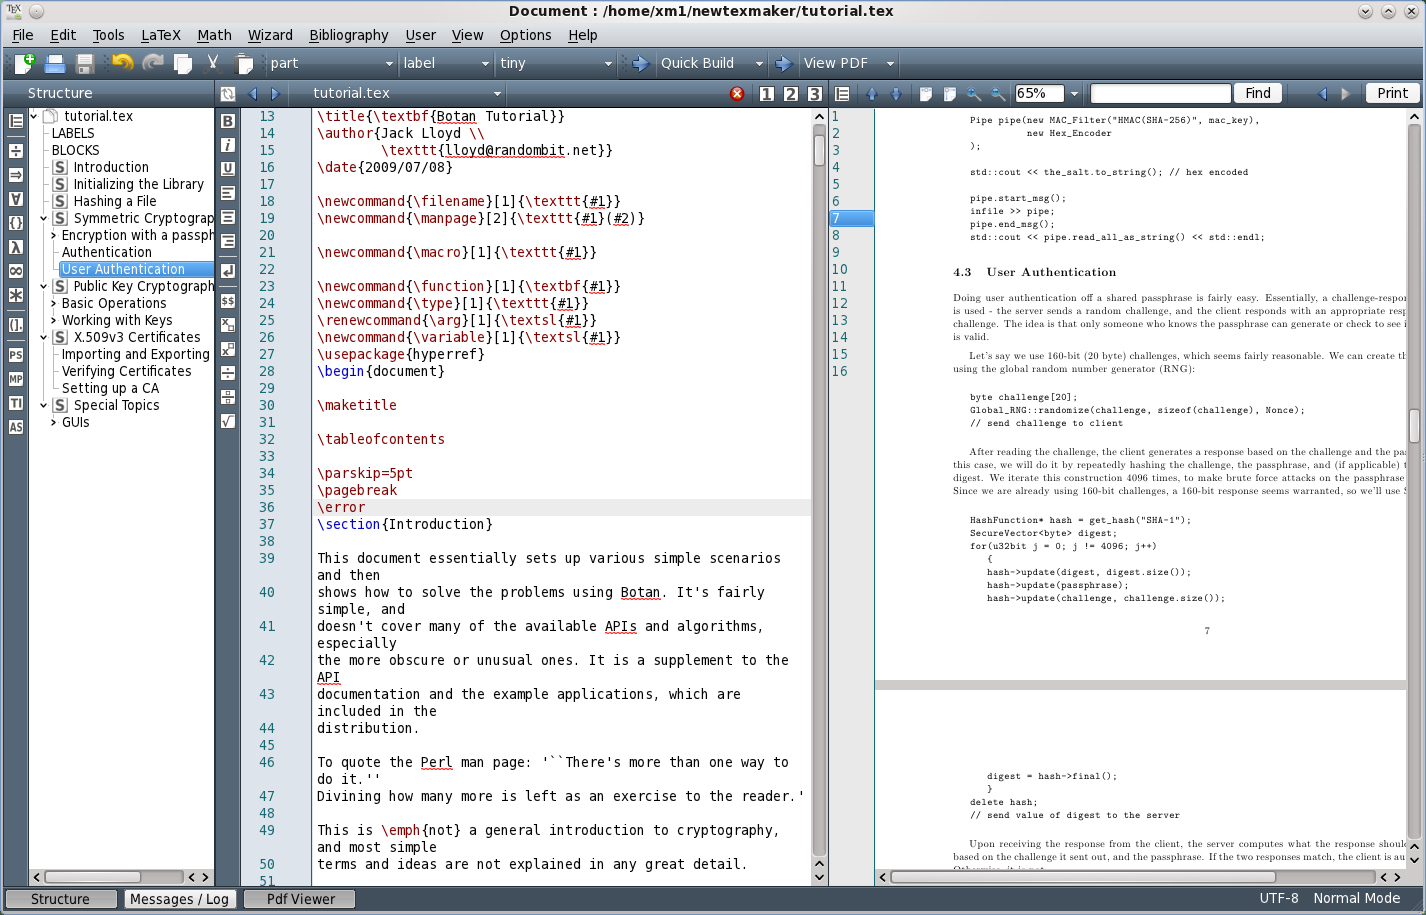
\includegraphics[width=\linewidth]{texmaker}\\
\textbf{Texmaker}
\end{figure}

\begin{figure}
\centering
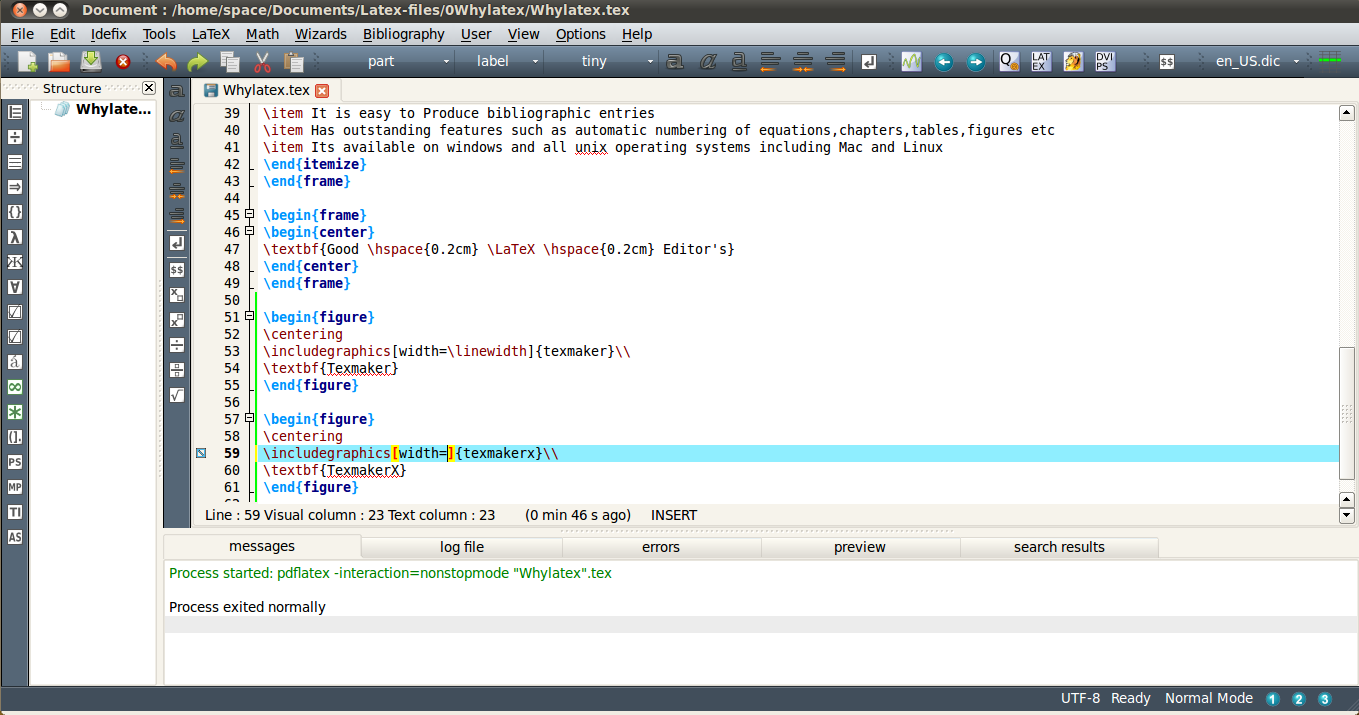
\includegraphics[width=\linewidth]{texmakerx}\\
\textbf{TexmakerX}
\end{figure}


\begin{figure}
\centering
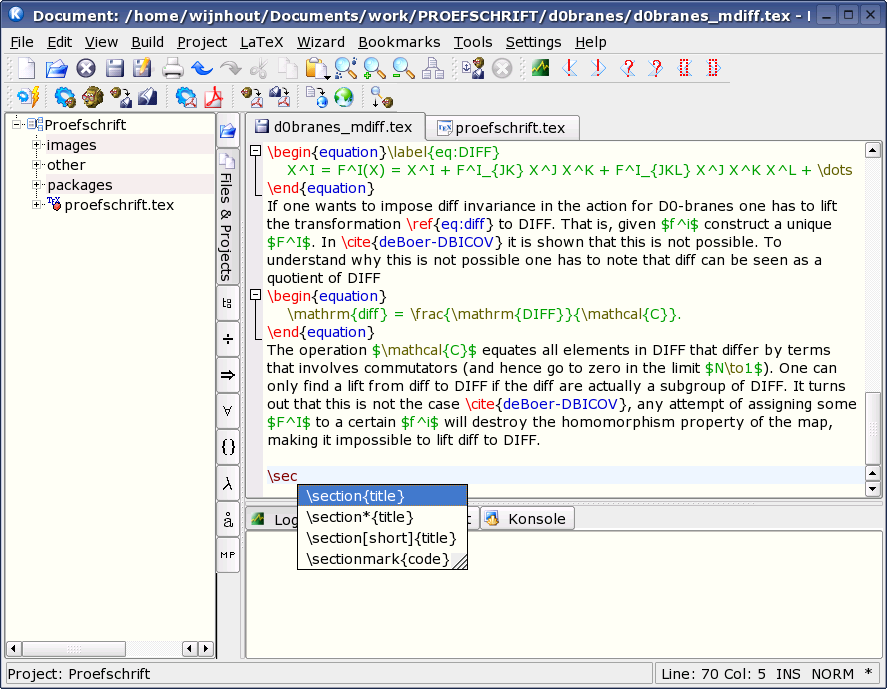
\includegraphics[width=\linewidth]{kile}\\
\textbf{Kile}
\end{figure}

\end{document}